\documentclass[12pt, titlepage]{article}

\usepackage{fullpage}
\usepackage[round]{natbib}
\usepackage{multirow}
\usepackage{booktabs}
\usepackage{tabularx}
\usepackage{graphicx}
\usepackage{float}
\usepackage{hyperref}
\hypersetup{
    colorlinks,
    citecolor=blue,
    filecolor=black,
    linkcolor=red,
    urlcolor=blue
}

\input{../../Comments.text}
\input{../../Common.text}

\newcounter{acnum}
\newcommand{\actheacnum}{AC\theacnum}
\newcommand{\acref}[1]{AC\ref{#1}}

\newcounter{ucnum}
\newcommand{\uctheucnum}{UC\theucnum}
\newcommand{\uref}[1]{UC\ref{#1}}

\newcounter{mnum}
\newcommand{\mthemnum}{M\themnum}
\newcommand{\mref}[1]{M\ref{#1}}

\begin{document}

\title{Module Guide for \progname{}} 
\author{\authname}
\date{\today}

\maketitle

\pagenumbering{roman}

\section{Revision History}

\begin{tabularx}{\textwidth}{p{3cm}p{2cm}X}
\toprule {\bf Date} & {\bf Version} & {\bf Notes}\\
\midrule
Date 1 & 1.0 & Notes\\
Date 2 & 1.1 & Notes\\
\bottomrule
\end{tabularx}

\newpage

\section{Reference Material}

This section records information for easy reference. 

\subsection{Abbreviations and Acronyms}

\renewcommand{\arraystretch}{1.2}
\begin{tabular}{l l} 
  \toprule		
  \textbf{symbol} & \textbf{description}\\
  \midrule 
  AC & Anticipated Change\\
  DAG & Directed Acyclic Graph \\
  M & Module \\
  MG & Module Guide \\
  OS & Operating System \\
  R & Requirement\\
  SC & Scientific Computing \\
  SRS & Software Requirements Specification\\
  \progname & Explanation of program name\\
  UC & Unlikely Change \\
  \wss{etc.} & \wss{...}\\
  \bottomrule
\end{tabular}\\

\newpage

\tableofcontents

\listoftables

\listoffigures

\newpage

\pagenumbering{arabic}

\section{Introduction}

Spectropica is a customizable educational game suite designed to support
autistic Learners through activities focused on routine sequencing,
functional communication, and short-term memory. Care Team Members (CTMs),
including parents, caregivers, and educators, can personalize gameplay
and review recorded performance. The system provides educational practice,
not clinical assessment or diagnosis.

This Module Guide (MG) describes Spectropica's modular architecture. The
design follows the principle of information hiding described by
\citet{Parnas1972a}: each module hides a design decision that may change
independently of other parts of the system. This approach aims to limit
dependencies and support implementation, testing, and maintenance.

The decomposition follows the principles outlined by
\citet{ParnasEtAl1984}:
\begin{itemize}
  \item Design decisions likely to change independently should be
    hidden within separate modules.
  \item Each data structure should be implemented and managed by a
    single module.
  \item Other modules should access that data through the owning
    module's defined interface rather than its internal implementation.
\end{itemize}

These principles support changes to educational content, personalization,
and reporting while limiting their effects on unrelated functionality.
The decomposition also provides a basis for connecting requirements to
the software architecture.

The MG builds on the
\href{https://github.com/meena-alomran/game-n-grow/blob/main/docs/SRS-IEEE/SRS.tex}
  {Software Requirements Specification (SRS)} and complements the
\href{https://github.com/meena-alomran/game-n-grow/blob/main/docs/Design/SoftDetailedDes/MIS.tex}
  {Module Interface Specification (MIS)}. The SRS defines required behaviour
and quality attributes; the MIS specifies individual module interfaces.

The intended readers are:
\begin{itemize}
  \item \textbf{New project members:} To understand the architecture
    and locate modules responsible for particular functionality.
  \item \textbf{Maintainers:} To identify modules affected by a
    proposed change and understand their dependencies.
  \item \textbf{Designers and developers:} To evaluate the
    decomposition, check requirement coverage, and coordinate
    implementation and integration.
\end{itemize}

Section~\ref{SecChange} identifies anticipated and unlikely changes.
Section~\ref{SecMH} presents the module hierarchy, and
Section~\ref{SecConnection} explains the design decisions connecting
requirements to the architecture. Section~\ref{SecMD} describes the
modules. Section~\ref{SecTM} traces requirements and anticipated changes
to modules. Section~\ref{SecUse} presents module dependencies through
the uses hierarchy. The remaining sections address user interfaces,
communication protocols, database design, the development timeline,
and generative AI use disclosure.

Project documentation and implementation are available at
\url{https://github.com/meena-alomran/game-n-grow}.

\section{Anticipated and Unlikely Changes} \label{SecChange}

This section identifies decisions that may change during development or
maintenance and stable assumptions on which the architecture relies.
The anticipated changes cover SRS Section 12 and additional design choices.
Module names refer to the hierarchy in Section~\ref{SecMH} and the
responsibilities in Section~\ref{SecMD}.

\subsection{Anticipated Changes} \label{SecAchange}

These entries concern changes to supported capabilities and design choices,
not ordinary runtime selections. Each entry identifies its responsible
module or explains why a coordinated change spans several modules.
Section~\ref{SecTM} records the corresponding traceability mappings.

\begin{description}

\item[\refstepcounter{acnum} \actheacnum
\label{acHardware}:]
\textbf{Platform and device interfaces.}
Supported operating-system and input interfaces may change across iPadOS and Android tablets and browser access. Device access is hidden behind the Hardware-Hiding interface. Platform changes that also require interface adaptation are coordinated with the affected presentation modules. This covers SRS LC7 and relates to SC1 and SC2.

\textit{Responsible module(s):} Hardware-Hiding.

\item[\refstepcounter{acnum} \actheacnum
\label{acGameImplementation}:]
\textbf{Game content and task rules.}
Content, available difficulty levels, and task-completion rules may change following evaluation. Game-specific behaviour is encapsulated within Game Session, alongside the common session lifecycle, rather than introducing additional top-level modules. This covers SRS LC1; changes to supported configuration fields also involve the configuration owners below.

\textit{Responsible module(s):} Game Session.

\item[\refstepcounter{acnum} \actheacnum
\label{acAdditionalGames}:]
\textbf{Supported Game collection.}
New Games add task behaviour within Game Session and a selectable entry in Game Suite. Game Personalization and Dashboard are affected only when the addition introduces new setting types or performance measures. This coordinated extension is an exception to a single-module mapping because execution, selection, configuration, and reporting have distinct responsibilities. This covers SRS LC8.

\textit{Responsible module(s):} Game Session and Game Suite.

\item[\refstepcounter{acnum} \actheacnum
\label{acCustomization}:]
\textbf{Learner-specific configuration rules.}
Supported per-Game settings and Game authorizations may evolve. Game Personalization owns the Learner-specific assignment and validation of these settings. Adding a new setting may also change its consumption within Game Session; this interface change must be coordinated. This covers the personalization portion of SRS LC2.

\textit{Responsible module(s):} Game Personalization.

\item[\refstepcounter{acnum} \actheacnum
\label{acTemplateOrganization}:]
\textbf{Template content and organization rules.}
Reusable configuration content, assignment, folders, and sharing rules may evolve while Templates remain variations of existing Games. Template owns these rules; File Import/Export owns only their external file representation. This covers SRS LC6 and the Template portion of LC2.

\textit{Responsible module(s):} Template.

\item[\refstepcounter{acnum} \actheacnum
\label{acUserInterface}:]
\textbf{Presentation and navigation.}
Game Suite owns Game selection, Game Session owns in-game interaction, and Dashboard owns performance views. CTM management views follow their corresponding account, profile, care team, personalization, and Template responsibilities. Charting owns chart rendering. This cross-cutting change intentionally maps to multiple modules because there is no separate general UI module in the decomposition. Each change is traced to the affected workflow. This covers SRS LC5 and the presentation portion of LC3.

\textit{Responsible module(s):} The module responsible for the affected user workflow.

\item[\refstepcounter{acnum} \actheacnum
\label{acDataStorage}:]
\textbf{Persistence technology and representation.}
Server storage, record mapping, backup, restoration, and permanent deletion mechanisms may change behind the Database interface. Higher-level modules retain ownership of domain rules, rather than accessing storage representations directly.

\textit{Responsible module(s):} Database.

\item[\refstepcounter{acnum} \actheacnum
\label{acPerformanceReporting}:]
\textbf{Performance measures and calculation rules.}
Calculation and filtering rules may change as CTMs identify useful measures. Dashboard owns these rules, while Charting renders the resulting values. If a new measure requires additional raw observations, Game Session recording and the Database record representation must also change. This justified exception preserves the separation of collection and analysis. Historical results must remain interpretable. This covers the calculation portion of SRS LC3.

\textit{Responsible module(s):} Dashboard.

\item[\refstepcounter{acnum} \actheacnum
\label{acRewards}:]
\textbf{Reward content and eligibility rules.}
Available items, unlock conditions, and alternative-item groupings may change while preserving Learner inventory relationships. This covers SRS LC4.

\textit{Responsible module(s):} Rewards \& Cosmetics.

\item[\refstepcounter{acnum} \actheacnum
\label{acDataExchange}:]
\textbf{Synchronization mechanisms.}
Local queueing, transfer, retry, and synchronization mechanisms may change without changing Game Session recording responsibilities. Storage and synchronization remain within Database as a single persistence boundary in this decomposition; their internal mechanisms can evolve behind its interface.

\textit{Responsible module(s):} Database.

\item[\refstepcounter{acnum} \actheacnum
\label{acExportFormat}:]
\textbf{Import and export file representations.}
Template file representations and Learner-data export formats may change. Template and Dashboard retain responsibility for selecting and authorizing the domain information; File Import/Export converts that information and validates imported file structure.

\textit{Responsible module(s):} File Import/Export.

\item[\refstepcounter{acnum} \actheacnum
\label{acAccountWorkflow}:]
\textbf{CTM account workflow.}
Registration validation, verification workflow, and account deletion/restoration rules may change. CTM Account coordinates these workflows while delegating credential and login-session mechanisms to Security.

\textit{Responsible module(s):} CTM Account.

\item[\refstepcounter{acnum} \actheacnum
\label{acAuthentication}:]
\textbf{Credential and login-session mechanisms.}
Password verification, encryption, and CTM login-session handling may change behind the Security interface without introducing Learner password-based login.

\textit{Responsible module(s):} Security.

\item[\refstepcounter{acnum} \actheacnum
\label{acDevicePairing}:]
\textbf{Learner device-pairing rules.}
Pairing-code generation, expiry, retry, lockout, and device-recognition rules may change while preserving the relationship between a paired device and a Learner profile.

\textit{Responsible module(s):} Device Pairing.

\item[\refstepcounter{acnum} \actheacnum
\label{acAccessControl}:]
\textbf{Care team permissions.}
Membership and CTM permission rules may evolve. Care Team answers permission queries; the module performing an operation applies the answer before proceeding. Learner Game authorization remains a separate Game Personalization responsibility.

\textit{Responsible module(s):} Care Team.

\item[\refstepcounter{acnum} \actheacnum
\label{acExternalCommunication}:]
\textbf{External message-delivery mechanisms.}
The email provider and message formatting may change behind a delivery interface. Account and care team workflows retain responsibility for deciding when messages are required.

\textit{Responsible module(s):} External Communication.

\end{description}

\subsection{Unlikely Changes} \label{SecUchange}

The following assumptions are expected to remain stable. Designing for
their complete replacement would introduce complexity without a clear
project benefit. A change to these assumptions could require revisions
across several modules. These entries summarize relevant stable
characteristics from SRS Section 13.

\begin{description}

\item[\refstepcounter{ucnum} \uctheucnum
\label{ucPurpose}:]
\textbf{Educational Games as the primary experience.}
Spectropica will remain an educational game suite supporting autistic
Learners. Replacing Games with an unrelated primary activity would
substantially change its purpose and architecture. This is consistent
with SRS ULC5.

\item[\refstepcounter{ucnum} \uctheucnum
\label{ucUserRoles}:]
\textbf{Distinct Learner and CTM responsibilities.}
Learners participate in Games, while authorized CTMs manage profiles,
configurations, and performance information. Individual memberships
and permissions may change without replacing this role structure.
This is consistent with SRS ULC1 and ULC3.

\item[\refstepcounter{ucnum} \uctheucnum
\label{ucCoreWorkflow}:]
\textbf{Learner-specific configuration and recording.}
Authorized CTMs configure activities for identifiable Learner profiles;
Learners participate in Games, and resulting session records remain
associated with the correct Learner and Game for review. Configuration
does not imply that a CTM must prepare every individual session.
This is consistent with SRS ULC2, ULC4, and ULC6.

\item[\refstepcounter{ucnum} \uctheucnum
\label{ucNonClinical}:]
\textbf{Non-clinical purpose.}
Performance records describe outcomes within Games rather than diagnose
conditions or establish broader developmental conclusions. Adopting a
clinical purpose would require reconsidering requirements, validation,
and architecture. This is consistent with SRS ULC8.

\end{description}

\section{Module Hierarchy} \label{SecMH}

This section provides an overview of the module design. Modules are summarized
in a hierarchy decomposed by secrets in Table \ref{TblMH}. The modules listed
below, which are leaves in the hierarchy tree, are the modules that will
actually be implemented.

\begin{description}
\item [\refstepcounter{mnum} \mthemnum \label{mHH}:] Hardware-Hiding Module
\item ...
\end{description}


\begin{table}[h!]
\centering
\begin{tabular}{p{0.3\textwidth} p{0.6\textwidth}}
\toprule
\textbf{Level 1} & \textbf{Level 2}\\
\midrule

{Hardware-Hiding Module} & ~ \\
\midrule

\multirow{7}{0.3\textwidth}{Behaviour-Hiding Module} & ?\\
& ?\\
& ?\\
& ?\\
& ?\\
& ?\\
& ?\\ 
& ?\\
\midrule

\multirow{3}{0.3\textwidth}{Software Decision Module} & {?}\\
& ?\\
& ?\\
\bottomrule

\end{tabular}
\caption{Module Hierarchy}
\label{TblMH}
\end{table}

\section{Connection Between Requirements and Design}
\label{SecConnection}

This section assigns design responsibilities to the modules in
Section~\ref{SecMD} and explains how those choices support the SRS and
Hazard Analysis. Requirement identifiers refer to the completed IEEE SRS
linked in the Introduction. These decisions refine the existing module
boundaries; they do not introduce additional top-level modules.

\subsection*{Learner Access and CTM Management}

CTM Account coordinates registration, login, and account lifecycle
operations. Security verifies credentials and manages CTM login sessions.
Device Pairing associates devices with Learner profiles through pairing
codes, so Learners do not need a separate username/password login or a
CTM sign-in before each session. These responsibilities support FR-CTM-4
and FR-DEV-1--5 while separating account workflow from credential mechanisms.

Care Team owns membership and CTM permission decisions. Each management
module checks the applicable permission before performing an operation;
hiding controls alone does not authorize access. Game Personalization
owns Learner Game authorizations, Game Suite displays authorized choices,
and Game Session checks authorization before starting a selected Game.
This supports FR-TEAM-4, FR-TEAM-7, FR-PERS-1, and FR-PLAY-1. CTM management
operations remain separate from Learner-facing Game selection and play.

\subsection*{Game Customization and Configuration}

Game Personalization owns Learner-specific settings and authorizations;
Template owns reusable variations and their assignment. Game Personalization owns the supported per-Game setting definitions;
Template uses that configuration interface when validating reusable values.
Game Session consumes a validated configuration and owns the task rules
that interpret it. Configuration validation does not call back into Game
Session, avoiding a circular dependency. File Import/Export checks
imported file structure before Template performs domain validation.
This supports FR-PERS-1--4, FR-TMPL-4, FR-TMPL-6, and SR-15.

Game Session loads an effective configuration for the correct Learner and
Game before entering the ready state. Invalid or unavailable required
settings prevent the Game from starting; the Learner receives the calm
return-to-suite action required by SR-7. A failed edit retains the previous
saved configuration and reports the failure to the CTM, consistent with
SR-13. Template provides the affected-Learner preview and confirmation
required by SR-14 before assignment changes.

Game-specific activities are internal components of Game Session and use
its common lifecycle interface. This keeps each Game's task rules separate
internally while maintaining the top-level decomposition. Configuration
management remains distinct from executing those rules, limiting the
impact of changes to an individual Game.

\subsection*{Learner Wellbeing and Accessible Gameplay}

Game Session provides common readiness, pause, resume, restart, exit, and
error-handling behaviour across Games. Game Personalization and Template
validate sensory settings before saving them; Game Session applies those
settings and enforces runtime presentation constraints. Game-specific
content must also satisfy the flashing restriction. These responsibilities
support SR-4--7, SR-11, and FR-PLAY-2 and FR-PLAY-5--7.

A common lifecycle prevents individual Games from omitting participation
controls or starting audio and animation before the Learner is ready.
Sensory defaults follow SR-4, and CTM customization cannot override a
mandatory safety constraint. This preserves Learner control under SRS ULC7
without introducing a separate safety module.

\subsection*{Session Recording and Performance Reporting}

Game Session owns the active session state and constructs records containing
the Learner, Game, settings used, and outcome. Database owns durable records
and unsynchronized copies. Dashboard reads records to compute and filter
performance information, Charting renders the selected representation, and
File Import/Export formats the records selected for export. This separates
record collection, persistence, interpretation, and rendering, supporting
FR-DATA-2--7 and SR-16.

Only completed sessions contribute to completion-based performance averages.
Aborted, restarted, and interrupted sessions remain visible in history with
their outcome but are excluded from those averages. Restarting closes the
current attempt and begins a new session. A crash or a connection failure
that actually terminates play produces an incomplete session; temporary
connection loss alone does not invalidate a session that continues and
finishes normally. This interpretation implements SR-8 alongside SR-9.
The session representation must distinguish interrupted outcomes in addition
to the completed, aborted, and restarted outcomes already listed in the SRS.

Dashboard does not silently compare unlike metrics or difficulty settings;
records retain the context needed to interpret results. Reported results
remain descriptions of Game performance, not clinical or developmental
assessments. Changing dashboard presentation does not rewrite raw records.

\subsection*{Data Persistence and Connectivity}

Database provides the persistence boundary for server records, local queues,
synchronization, backups, and restoration. Domain modules request operations
through its interface rather than accessing tables or queues directly.
Although this boundary contains several mechanisms, they share responsibility
for preserving records across storage locations and failures. The decomposition
retains this grouping to match the current module hierarchy; its internal
mechanisms remain distinct and are not exposed to gameplay modules.

Network access is required for account, pairing, care team, and shared-data
management operations. During a connection loss, Game Session may continue
an ongoing Game and Game Suite may offer previously authorized Games only
when the required Game resources and settings are already available locally.
A Game requiring an uncached resource cannot start offline. This limited
offline support follows SR-9 while retaining SC3's network dependence for
management operations; it does not promise unrestricted offline use.

Database retains queued session records across application restarts and
removes them only after confirmed server persistence. Retries use the session
identifier to avoid duplicate records. Pending synchronization is distinct
from confirmed server storage. After reconnection, cached authorizations and
settings are refreshed before subsequent Game starts. Immediate remote
revocation on a disconnected device is not assumed.

For settings, Templates, and equipped items, the owning module reports success
only after Database confirms the write. Failed changes retain the previous
saved values, as required by SR-13. Database also owns backup and restoration
mechanisms under SR-17. These choices keep persistence failure handling out
of game-specific task logic while exposing enough status for appropriate
feedback.

\subsection*{Data Privacy and Lifecycle Management}

Learner Profile coordinates profile deletion and restoration; CTM Account
coordinates account deletion and restoration. Care Team updates membership
and ownership relationships, and Device Pairing unlinks affected devices.
Database performs scheduled permanent deletion, synchronization, and removal
from backups. This divides lifecycle policy from storage mechanics while
supporting FR-LRN-4--8, FR-CTM-5--6, and SR-18.

The design retains the 30-day grace period stated in SRS Section 7.3 rather
than introducing another duration. Restoration cancels pending permanent
deletion during that period. Permanent deletion covers the affected records
and backups according to the same authoritative lifecycle policy. Care Team
must preserve a valid Primary CTM for active Learner profiles when an account
is removed; account deletion does not itself delete those profiles.

Unlinked devices lose profile access and clear associated local data when
unlinking is processed locally. A disconnected device cannot receive a remote
unlink immediately, so the next successful connection must reconcile device
status before further profile access or session uploads. A stale upload must
not recreate a deleted profile. Export before profile deletion remains an
authorized Primary CTM operation, with File Import/Export formatting the
selected data. These rules support the existing privacy obligations without
claiming instantaneous remote erasure from an offline device.

The responsibilities above determine the module mappings in
Section~\ref{SecTM}. The MIS must express the same ownership, failure outcomes,
and state transitions, and the uses hierarchy must include the dependencies
needed to obtain the stated services.

\section{Module Decomposition} \label{SecMD}

Modules are decomposed according to the principle of ``information hiding''
proposed by \citet{ParnasEtAl1984}. The \emph{Secrets} field in a module
decomposition is a brief statement of the design decision hidden by the
module. The \emph{Services} field specifies \emph{what} the module will do
without documenting \emph{how} to do it. For each module, a suggestion for the
implementing software is given under the \emph{Implemented By} title. If the
entry is \emph{OS}, this means that the module is provided by the operating
system or by standard programming language libraries.  \emph{\progname{}} means the
module will be implemented by the \progname{} software.

Only the leaf modules in the hierarchy have to be implemented. If a dash
(\emph{--}) is shown, this means that the module is not a leaf and will not have
to be implemented.

\subsection{Hardware Hiding Modules (\mref{mHH})}

\begin{description}
\item[Secrets:]The data structure and algorithm used to implement the virtual
  hardware.
\item[Services:]Serves as a virtual hardware used by the rest of the
  system. This module provides the interface between the hardware and the
  software. So, the system can use it to display outputs or to accept inputs.
\item[Implemented By:] OS
\end{description}

\subsection{Behaviour-Hiding Module}

\begin{description}
\item[Secrets:]The contents of the required behaviours.
\item[Services:]Includes programs that provide externally visible behaviour of
  the system as specified in the software requirements specification (SRS)
  documents. This module serves as a communication layer between the
  hardware-hiding module and the software decision module. The programs in this
  module will need to change if there are changes in the SRS.
\item[Implemented By:] --
\end{description}

\subsubsection{Input Format Module (\mref{mInput})}

\begin{description}
\item[Secrets:]The format and structure of the input data.
\item[Services:]Converts the input data into the data structure used by the
  input parameters module.
\item[Implemented By:] [Your Program Name Here]
\item[Type of Module:] [Record, Library, Abstract Object, or Abstract Data Type]
  [Information to include for leaf modules in the decomposition by secrets tree.]
\end{description}

\subsubsection{Etc.}


\subsection{Software Decision Module}

\begin{description}
\item[Secrets:] The design decision based on mathematical theorems, physical
  facts, or programming considerations. The secrets of this module are
  \emph{not} described in the SRS.
\item[Services:] Includes data structure and algorithms used in the system that
  do not provide direct interaction with the user. 
  % Changes in these modules are more likely to be motivated by a desire to
  % improve performance than by externally imposed changes.
\item[Implemented By:] --
\end{description}

\subsubsection{Etc.}

\section{Traceability Matrix} \label{SecTM}

This section shows two traceability matrices: between the modules and the
requirements and between the modules and the anticipated changes.

% the table should use mref, the requirements should be named, use something
% like fref
\begin{table}[H]
\centering
\begin{tabular}{p{0.2\textwidth} p{0.6\textwidth}}
\toprule
\textbf{Req.} & \textbf{Modules}\\
\midrule
R1 & \mref{mHH}, \mref{mInput}, \mref{mParams}, \mref{mControl}\\
R2 & \mref{mInput}, \mref{mParams}\\
R3 & \mref{mVerify}\\
R4 & \mref{mOutput}, \mref{mControl}\\
R5 & \mref{mOutput}, \mref{mODEs}, \mref{mControl}, \mref{mSeqDS}, \mref{mSolver}, \mref{mPlot}\\
R6 & \mref{mOutput}, \mref{mODEs}, \mref{mControl}, \mref{mSeqDS}, \mref{mSolver}, \mref{mPlot}\\
R7 & \mref{mOutput}, \mref{mEnergy}, \mref{mControl}, \mref{mSeqDS}, \mref{mPlot}\\
R8 & \mref{mOutput}, \mref{mEnergy}, \mref{mControl}, \mref{mSeqDS}, \mref{mPlot}\\
R9 & \mref{mVerifyOut}\\
R10 & \mref{mOutput}, \mref{mODEs}, \mref{mControl}\\
R11 & \mref{mOutput}, \mref{mODEs}, \mref{mEnergy}, \mref{mControl}\\
\bottomrule
\end{tabular}
\caption{Trace Between Requirements and Modules}
\label{TblRT}
\end{table}

\begin{table}[H]
\centering
\begin{tabular}{p{0.2\textwidth} p{0.6\textwidth}}
\toprule
\textbf{AC} & \textbf{Modules}\\
\midrule
\acref{acHardware} & \mref{mHH}\\
\acref{acInput} & \mref{mInput}\\
\acref{acParams} & \mref{mParams}\\
\acref{acVerify} & \mref{mVerify}\\
\acref{acOutput} & \mref{mOutput}\\
\acref{acVerifyOut} & \mref{mVerifyOut}\\
\acref{acODEs} & \mref{mODEs}\\
\acref{acEnergy} & \mref{mEnergy}\\
\acref{acControl} & \mref{mControl}\\
\acref{acSeqDS} & \mref{mSeqDS}\\
\acref{acSolver} & \mref{mSolver}\\
\acref{acPlot} & \mref{mPlot}\\
\bottomrule
\end{tabular}
\caption{Trace Between Anticipated Changes and Modules}
\label{TblACT}
\end{table}

\section{Use Hierarchy Between Modules} \label{SecUse}

In this section, the uses hierarchy between modules is
provided. \citet{Parnas1978} said of two programs A and B that A {\em uses} B if
correct execution of B may be necessary for A to complete the task described in
its specification. That is, A {\em uses} B if there exist situations in which
the correct functioning of A depends upon the availability of a correct
implementation of B.  Figure \ref{FigUH} illustrates the use relation between
the modules. It can be seen that the graph is a directed acyclic graph
(DAG). Each level of the hierarchy offers a testable and usable subset of the
system, and modules in the higher level of the hierarchy are essentially simpler
because they use modules from the lower levels.

\wss{The uses relation is not a data flow diagram.  In the code there will often
be an import statement in module A when it directly uses module B.  Module B
provides the services that module A needs.  The code for module A needs to be
able to see these services (hence the import statement).  Since the uses
relation is transitive, there is a use relation without an import, but the
arrows in the diagram typically correspond to the presence of import statement.}

\wss{If module A uses module B, the arrow is directed from A to B.}

\begin{figure}[H]
\centering
%\includegraphics[width=0.7\textwidth]{UsesHierarchy.png}
\caption{Use hierarchy among modules}
\label{FigUH}
\end{figure}

%\section*{References}

\section{User Interfaces}

\subsection{Learner Home Screen}

Figure~\ref{fig:learner-home} shows the proposed home screen on a paired
Learner device. \textbf{Play} opens the list of Games authorized for the
Learner. \textbf{Settings} opens a read-only view of the active Game settings.
An authorized Care Team Member (CTM) can change these settings from the
Dashboard. \textbf{Progress} shows a simple summary of completed activities.
Detailed session history and data exports are available through the CTM
Dashboard.

\begin{figure}[htbp]
    \centering
    \fbox{\begin{minipage}{0.62\linewidth}
        \centering
        \vspace{1em}
        {\Large\bfseries Spectropica\par}
        \vspace{1.25em}
        \fbox{\rule{0pt}{2em}\makebox[0.68\linewidth]{\large\bfseries Play}}\par
        \vspace{0.65em}
        \fbox{\rule{0pt}{1.75em}\makebox[0.32\linewidth]{Settings}}
        \hspace{0.35em}
        \fbox{\rule{0pt}{1.75em}\makebox[0.32\linewidth]{Progress}}\par
        \vspace{1em}
    \end{minipage}}
    \caption{Proposed Learner home screen wireframe.}
    \label{fig:learner-home}
\end{figure}

\subsection{Cashier Game Prototype}

Figure~\ref{fig:cashier-prototype} shows the cashier counter in the early
Godot prototype. The register has a numeric keypad, an amount display,
and a \textbf{Cash} button.

\begin{figure}[H]
    \centering
    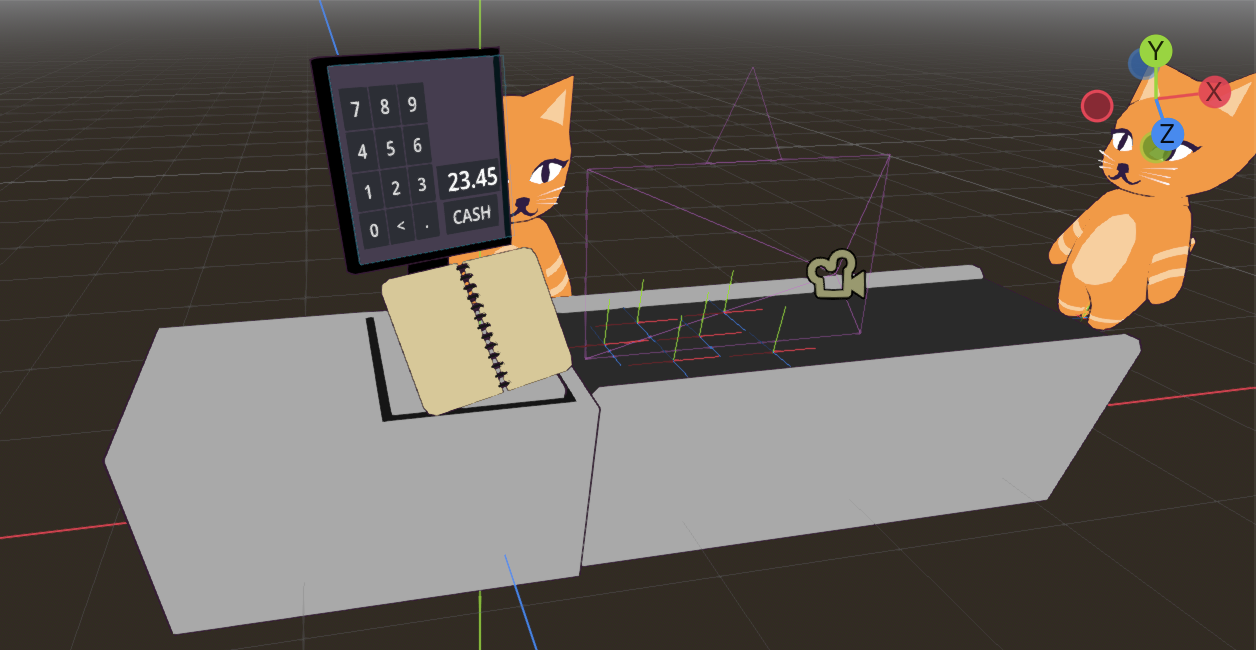
\includegraphics[width=0.9\linewidth]{CashierPrototype.png}
    \caption{Early cashier game prototype in the Godot editor.}
    \label{fig:cashier-prototype}
\end{figure}

\section{Design of Communication Protocols}

\wss{If there is communication between hardware and software, it may be necessary 
to explain the design of the communication protocol.  This section should be filled 
in with NA if it is not appropriate for a given project.}

\section{Database Design}

\wss{If a database is a significant component of the project, the database
design should be summarized here.  This section should be filled in with NA if
it is not appropriate for a given project.}

\section{Timeline}

Table~\ref{tab:module-timeline} proposes internal target dates and assigns
three modules to each team member. Each owner implements and tests their
modules. Owners pair up for integration tests when a workflow crosses module
boundaries.

\begin{table}[htbp]
\centering
\small
\begin{tabularx}{\textwidth}{@{}p{0.16\textwidth}p{0.19\textwidth}XX@{}}
\toprule
Target date & Owner & Module tasks & Verification activities \\
\midrule
8 Jan.\ 2027 & Omar Ghoneim
& Implement CTM Account, Database, and Security, including sign-in,
record storage, and access checks.
& Test sign-in and session expiry, denied access, and recovery after a
failed write. \\
\addlinespace
15 Jan.\ 2027 & Amirah Abdelrahman
& Implement Learner Profile, Care Team, and Device Pairing, including
profile management, invitations, and device linking.
& Test profile ownership transfer, permission changes, and expired or
reused pairing codes. \\
\addlinespace
22 Jan.\ 2027 & Marko Popovic
& Implement Game Suite, Game Session, and Rewards \& Cosmetics,
including the cashier game flow and session outcomes.
& Test game authorization, start and exit controls, interrupted sessions,
and reward eligibility. \\
\addlinespace
22 Jan.\ 2027 & Meena Al Omran
& Implement Game Personalization, Templates, and Dashboard, including
per-Learner settings, template previews, and session history.
& Test that settings persist, templates apply to the intended Learner,
and the dashboard distinguishes complete and incomplete sessions. \\
\addlinespace
29 Jan.\ 2027 & Maya Azar
& Implement File Import/Export, External Communication, and Charting,
including template validation, service failure handling, and progress plots.
& Test invalid imports, service failures, and agreement among charts,
dashboard counts, and exported records. \\
\addlinespace
12 Feb.\ 2027 & All owners
& Integrate CTM setup, device pairing, gameplay, and results.
& Run the end-to-end workflow, including a connection interruption,
resynchronization, and verification of permissions across devices. \\
\addlinespace
5 Mar.\ 2027 & All owners
& Run CTM usability sessions and Learner-facing proxy playtesting.
& Record usability findings, fix defects, rerun affected tests, and
capture results for the V\&V Report. \\
\bottomrule
\end{tabularx}
\caption{Proposed module implementation and verification timeline.}
\label{tab:module-timeline}
\end{table}

\section{Generative AI Use Disclosure}

This section records where the team used generative AI in preparing and
reviewing the Module Guide and how the team verified the resulting changes.

\subsection{AI Tools Used}

The team used ChatGPT (OpenAI GPT-6 Instant) and GPT-6 Luna in Visual Studio
Code.

\subsection{How and Where Used}

The team used AI to format \LaTeX{}, organize and check references, and review
grammar, spelling, and clarity throughout the guide.

The team used GPT-6 Luna in Visual Studio Code to format the traceability
matrices in Section~\ref{SecTM} and add hyperlinks and cross-references to the
corresponding modules. The team used ChatGPT to review
Sections~\ref{SecChange} and~\ref{SecConnection} for consistency with the
module architecture.

\subsection{Verification of AI-Generated Content}

The team checked AI-assisted changes against the Software Requirements
Specification (SRS), the Module Interface Specification (MIS), and the
project's module definitions to verify that the technical content and design
decisions remained consistent.

For Section~\ref{SecTM}, the team inspected the \LaTeX{} source and the
compiled PDF to verify the formatting and cross-references. The team tested
each hyperlink to confirm that it led to the intended module or section.

The team reviewed grammar and spelling suggestions to verify that they
preserved the intended technical meaning. The team is responsible for the
accuracy, completeness, consistency, and appropriateness of the final guide.

\newpage{}

\bibliographystyle {plainnat}
\bibliography{../../../refs/References}

\end{document}
